% !TeX root = ../main.tex

\section{Introduzione}
% situazione attuale (esistono team di sviluppo mobile in maggioli che non hanno automazione e non usano tecniche multiplatform) e cosa si vuole fare (si vuole fornire un modello di processo automatizzato e un esempio di utilizzo di strumenti multiplatform)

In questo capitolo vengono inizialmente descritte le motivazioni che hanno spinto l'azienda Maggioli S.p.A.\footnote{\href{https://www.maggioli.com/en-us}{https://www.maggioli.com/en-us}} a dedicare risorse per la ricerca e la sperimentazione nei campi delle applicazioni multipiattaforma e delle tecniche DevOps in ambito mobile. Successivamente sono indicati i requisiti del caso di studio industriale individuato, il quale può essere suddiviso in due macroaree:
\begin{itemize}
    \item definizione del processo di sviluppo per applicazioni multipiattaforma tramite l'adozione della cultura DevOps,
    \item sviluppo di una applicazione mobile multipiattaforma utilizzando il processo di sviluppo definito.
\end{itemize}

\section{Contesto aziendale}
% descrizione del contesto maggioli editore, editoria digitale e lo scopo della app
Tra i core business dell'azienda Maggioli S.p.A. è rimasto centrale il ruolo dell'editoria ma col trascorrere degli anni e il mutare delle esigenze dei clienti, i quali sono principalmente pubblica amministrazione (PA) e professionisti privati, come avvocati, architetti, commercialisti ed ingegneri edili, si è verificata una transizione verso il mondo digitale.

I servizi digitali erogati per la consultazione delle pubblicazioni hanno superato considerevolmente il formato cartaceo il quale rimane comunque un metodo secondario di consultazione disponibile seppur in forma molto ridotta. Per l'editoria digitale esiste in Maggioli una business unit dedicata, chiamata \textit{Digital Media}, il cui ruolo principale consiste nella realizzazione e manutenzione dei siti Web Maggioli dedicati alla ricerca e alla visualizzazione delle pubblicazioni digitali. I seguenti sono soltanto alcuni dei siti gestiti dal team \textit{Digital Media}: Biblioteca Digitale\footnote{\href{https://bibliotecadigitale.maggioli.it/}{https://bibliotecadigitale.maggioli.it/}}, Appalti \& Contratti\footnote{\href{https://www.appaltiecontratti.it/}{https://www.appaltiecontratti.it/}} e Periodici\footnote{\href{https://www.periodicimaggioli.it/}{https://www.periodicimaggioli.it/}}. La necessità principale è dunque quella di fare innovazione tramite lo sviluppo di una applicazione mobile in modo da fornire ai clienti Maggioli un nuovo metodo di accesso alle pubblicazioni che sia più accessibile e comodo. 

\begin{figure}[H]
    \centering
    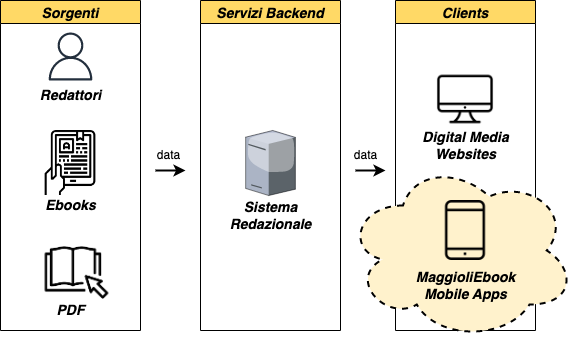
\includegraphics[width=0.7\textwidth]{img/contesto-aziendale.png}
    \caption{Schema del contesto aziendale in cui è collocato il caso di studio}
    \label{contesto-aziendale-fig}
\end{figure}

Le motivazioni che stanno alla base della scelta della cultura DevOps e delle applicazioni multipiattaforma per lo sviluppo di questo caso di studio sono comuni a qualsiasi tipologia di azienda: come descritto nei capitoli \ref{ch:devops} e \ref{ch:app-multiplatform} è possibile ottimizzare il processo di sviluppo diminuendo le risorse impiegante e quindi i costi ma allo stesso tempo si aumenta la qualità del software e la frequenza di rilascio i quali comportano una maggiore soddisfazione da parte dell'utente.

\section{Requisiti processo di sviluppo}
Considerando l'intero contesto aziendale esistono degli standard, consolidati con l'esperienza maturata nello sviluppo software, che devono essere adottati sia per quanto riguarda il processo di sviluppo che la scelta degli strumenti necessari.

L'obiettivo è riuscire a definire un modello di processo fortemente basato sugli standard aziendali ma adattato alle esigenze dello sviluppo di applicazioni mobile multipiattaforma e che possa essere introdotto nei team che si occupano di applicazioni mobile. I principali standard aziendali riguardanti gli strumenti e le tecnologie che devono essere adottati sono:

\begin{itemize}
    \item \textbf{GitLab}\footnote{\href{https://about.gitlab.com/}{https://about.gitlab.com/}} (\textit{DVCS/CI Server})- Le funzionalità necessarie al versionamento del codice, alla collaborazione/pianificazione e alla automazione (Sezione \ref{devops-tools-sec}) sono tutte soddisfatte dalla piattaforma cloud GitLab con la quale è presente una sottoscrizione di piano di licenza aziendale.
    \item \textbf{SonarQube}\footnote{\href{https://www.sonarqube.org/}{https://www.sonarqube.org/}} (\textit{Vulnerability Management System}) - Questo servizio self-hosted è reso disponibile a tutti i team aziendali e permette di soddisfare gran parte dei task di Continuous Inspection. Grazie a SonarQube è possibile effettuare l'analisi statica del codice, validare il rispetto di determinate policy aziendali e visualizzare dashboard sullo stato delle scansioni.
    \item \textbf{Renovate}\footnote{\href{https://docs.renovatebot.com/}{https://docs.renovatebot.com/}} (\textit{Dependency Management}) - Strumento utilizzato per automatizzare la gestione delle dipendenze dei progetti. 
\end{itemize}

La pipeline standard a livello aziendale, base di partenza per la definizione della pipeline per applicazioni mobile multipiattaforma, rispetta a pieno tutte le considerazioni fatte nel capitolo \ref{ch:devops} per tutte le tecniche di automazione indicate (fig. \ref{ci-inspection-pipeline}). Tramite l'adattamento delle fasi di integration, delivery e inspection di questa pipeline con le necessità dello sviluppo mobile indicate nei capitoli \ref{ch:sdlc} e \ref{ch:app-multiplatform} si ottengono i seguenti requisiti e dunque la pipeline obiettivo da realizzare:

\begin{itemize}
    \item \textbf{R1} - Continuous Integration
    \begin{itemize}
        \item \textbf{R1.1} - Stage di compilazione, testing e packaging con i relativi sotto-task per entrambe le piattaforme Android e iOS.
        \item \textbf{R1.2} - L'output dell'ultimo stage deve essere un pacchetto contenente l'applicazione da passare come artefatto alla fase successiva di delivery.
        \item \textbf{R1.3} - Utilizzo del sistema aziendale di gestione automatica delle dipendenze Renovate.
    \end{itemize}
    \item \textbf{R2} - Continuous Delivery
    \begin{itemize}
        \item \textbf{R2.1} - Stage di stabilizzazione suddivisi tra \textit{Alpha} e \textit{Beta} per il testing interno ed esterno tramite gli appositi servizi forniti da Google e Apple: Google Play Console per l'applicazione Android e Testflight per l'applicazione iOS.
        \item \textbf{R2.2} - L'applicazione soggetta a stabilizzazione è data in input dalla fase precedente di integrazione.
        \item \textbf{R2.3} - Stage di pubblicazione sui relativi marketplace Google Play Store o App Store. L'applicazione soggetta a pubblicazione deriva dalla terminazione con successo della fase di stabilizzazione e si trova già sui portali utilizzati.
    \end{itemize}
    \item \textbf{R3} - Continuous Inspection
    \begin{itemize}
        \item \textbf{R3.1} - Stage di analisi statica e analisi delle dipendenze per entrambe le piattaforme.
        \item \textbf{R3.2} - Utilizzo del sistema aziendale di gestione delle vulnerabilità centralizzato SonarQube.
    \end{itemize}
\end{itemize}

\begin{figure}[H]
    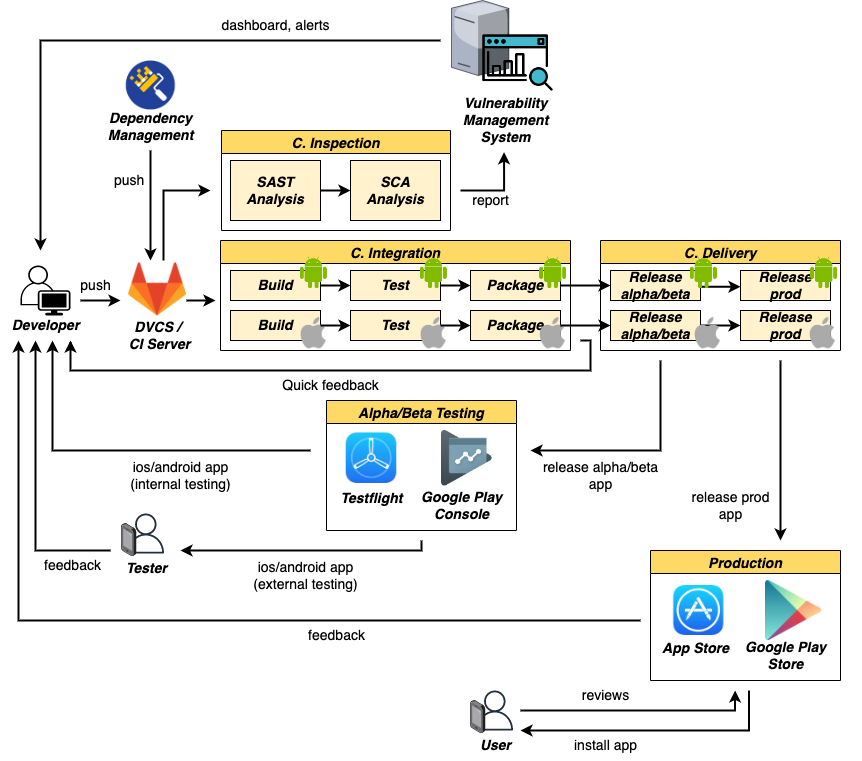
\includegraphics[width=1\textwidth]{img/full-cicd.png}
    \caption{Schema globale del processo di sviluppo automatizzato che si intende realizzare}
    \label{full-cicd}
\end{figure}

\section{Requisiti applicazione multipiattaforma}
% requisiti della applicazione da sviluppare, come sono stati identificati, ... (reader, epub, segnalibri, ecc)